\providecommand{\hciso}{\mathbb{I}}   %
\providecommand{\csp}{\cdot\!\lrcorner}   %
\providecommand{\qcOne}{\mathbf{1}}   %
\providecommand{\qcTwo}{\mathbf{2}}   %

\section{柔性加权极限}\label{sec:flexible-weighted-limits}

本节旨在引入一类特殊的、取值于单纯集的权，与其相关联的诸\trWeightedLimit{}概念
在同伦意义上表现良好。我们从 2-范畴理论中借来一个词，把这些权称为%
\emph{\trFlexible}。全部\trCosmologicalLimitNotions{}都可以理解为\trFlexibleWeightedLimit{}。
事实上，我们将证明∞-宇宙容有全部\trFlexibleWeightedLimit{}，因为它们可以由公理化的宇宙论
极限构造出来。在 6.3 节中，我们将利用这一观察，以更有效率的方式对新构造的%
\trInfinityCosmos{}验证极限公理。

粗略地说，\trFlexibleWeightedLimit{}是这样一类\trSimpliciallyEnrichedLimit：其中出现在%
\trCone{}里的诸单纯形，相对于\trDiagram{}形状是自由附接的。通常的「锥形」锥
涉及由两条锥腿与\trDiagram{}中一支箭头构成的交换三角形。这种交换性在柔性权所
规定的锥形状中是不被允许的；取而代之的是，一个由 0-箭头构成的\trDiagram{}可以
在更高维胞腔存在的意义下交换。若你对富集范畴理论中的加权极限概念还不熟悉，
我们建议在继续之前先阅读 A.4 节至 A.6 节。

\begin{definition}[作为射影胞腔复形的柔性权]\label{def:flexible-weights}
对一个\trSimplicialCategory{} $A$，考虑由诸\trSimplicialFunctor{}——称为%
\textbf{权}（weight）——与诸单纯自然变换构成的范畴 $sSet^{A}$。
\begin{itemize}
\item 对任意 $n\geq 0$ 与 $A$ 的对象 $a$，形如下式的单纯自然变换
\[
\partial\Delta[n]\times A(a,-)\hookrightarrow\Delta[n]\times A(a,-)
\]
称为一个\textbf{$a$ 处的射影 $n$-胞腔}（projective $n$-cell at $a$）。
\item 一支能表为诸射影胞腔之\trCoproduct{}的\trPushout{}的可数复合的单纯自然变换
$\alpha\colon V\hookrightarrow W$，称为一个\textbf{射影胞腔复形}（projective
cell complex）。
\item 一个权 $W$ 是\textbf{\trFlexible}（flexible），当且仅当
$\varnothing\hookrightarrow W$ 是一个射影胞腔复形。
\end{itemize}
取值于某个\trInfinityCosmos{}中的一张\trDiagram{} $F\colon A\to\mathcal{K}$ 的%
\textbf{\trFlexibleWeightedLimit}（flexible weighted limit），是 A.6 节意义下的一个%
\trWeightedLimit，其权 $W\colon A\to sSet$ 是\trFlexible。
\end{definition}

\begin{remark}\label{rem:projective-cell-complexes}
由于单纯集的任何单态射 $U\hookrightarrow V$ 都能分解为诸边界包含
$\partial\Delta[n]\hookrightarrow\Delta[n]$ 之\trCoproduct{}的\trPushout{}的可数复合，射影胞腔
复形类也可以描述为 $sSet^{A}$ 中那些能表为如下形状之单态射——对某
$U\hookrightarrow V\in sSet$ 与 $a\in A$ 而言的
$U\times A(a,-)\hookrightarrow V\times A(a,-)$——之\trCoproduct{}的\trPushout{}的可数复合的映射
所构成的类。
\end{remark}

\begin{example}[余张量是柔性的]\label{exa:cotensors-flexible}
回忆 A.4 节：\trInfinityCosmos{} $\mathcal{K}$ 中的\trInfinityCategory{} $A$
与单纯集 $U$ 的\trCotensor{}是对象 $A^{U}\in\mathcal{K}$，它由单纯自然同构
\[
\mathrm{Fun}(X,A^{U})\cong\mathrm{Fun}(X,A)^{U}
\]
刻画。这个对象可以看作\trDiagram{} $A\colon\qcOne\to\mathcal{K}$ 以
$U\colon\qcOne\to sSet$ 加权的\trLimit。这个权由在 $\qcOne$ 的唯一对象处的一个形状为
$\varnothing\hookrightarrow U$ 的广义射影胞腔定义。
\end{example}

回忆 A.5 节：\trDiagram{} $F\colon A\to\mathcal{K}$ 的\textbf{锥形极限}%
（conical limit）是以终权 $*\colon A\to sSet$ 加权的\trLimit。

\begin{example}[积是柔性的]\label{exa:products-flexible}
锥形积也定义\trFlexibleWeightedLimit{}，其构造方式是在指标集的每个对象处各附上一个射影
0-胞腔。
\end{example}

\begin{nonexample}\label{nex:conical-not-flexible}
由任何含非恒同箭头的 1-范畴作指标的锥形极限都\emph{不}是柔性的，因为锥形锥的
诸条锥腿被要求在\trDiagram{}的每支 0-箭头之上定义严格交换的三角形。柔性权的
规格允许我们自由附接任意维数的 $n$-箭头，却不提供任何强求诸 $n$-箭头之%
\trDiagram{}严格交换的机制——只容许在更高维胞腔存在意义下的交换。
\end{nonexample}

\begin{example}[逗号是柔性的]\label{exa:commas-flexible}
在\trInfinityCosmos{} $\mathcal{K}$ 中，\trDiagram{}
$\csp\to\mathcal{K}$——由\trCospan
\[
C\xrightarrow{\ \ g\ \ }A\xleftarrow{\ \ f\ \ }B
\]
给出——以\trDiagram{} $\csp\to sSet$——由\trCospan
\[
\qcOne\xrightarrow{\ \ 1\ \ }\qcTwo\xleftarrow{\ \ 0\ \ }\qcOne
\]
给出——加权的\trLimit，就是\trCommaInfinityCategory{}
$\mathrm{Hom}_{A}(f,g)$（见例 A.6.14）。由于这个权可以这样构造：先在\trCospan{}的
两个角处各附上一个射影 0-胞腔，再在\trCospan{}的\trTerminal{}对象处附上一个射影
1-胞腔，所以逗号对象是\trFlexibleWeightedLimit{}。
\end{example}

\begin{digression}[论 2-范畴理论中的柔性极限]\label{dig:flexible-2-limits}
以柔性权加权的单纯极限，应当被理解为\textbf{柔性 2-极限}（flexible 2-limits）
的类比物，即由积、插入子、均衡化子与收缩（幂等的分裂）构造出的富集范畴式极限
[18]。由于我们把柔性权定义为\trCoproduct{}的\trPushout{}的可数复合——而非（对其结果再取）收缩
——\cref{def:flexible-weights}的\trFlexibleWeightedLimit{}更精确地类比于\textbf{PIE 极限}%
（PIE limits），即仅由积、插入子与均衡化子构造出的极限。PIE 极限还包括同构
插入子、下降对象、逗号对象与 Eilenberg--Moore 对象，以及全部拟极限、松弛极限
与反松弛极限。许多重要的 2-范畴——例如由可及范畴与可及函子构成的 2-范畴——
不容有全部 2-范畴式极限，却容有全部 PIE 极限 [83]。

以 2-范畴 $A$ 为指标的柔性 2-极限之权，是图表 2-范畴 $\mathcal{C}at^{A}$ 上
一个模型结构中的余纤维性对象，该模型结构富集于 $\mathcal{C}at$ 上的\trFolkModelStructure；
PIE 权恰好是\emph{胞腔式的}余纤维性对象（见定义 C.2.4）。相应地，
\cref{def:flexible-weights}的射影胞腔复形恰好是 $sSet^{A}$ 上射影模型结构中的
胞腔式余纤维化。
\end{digression}

这暗示「PIE 极限」会是\cref{def:flexible-weights}的\trFlexibleWeightedLimit{}的一个更精确的
名字，对此我们并无异议。但向散居世界各地的澳大利亚 2-范畴理论学家致歉之余，
我们实在抵挡不住这个更富意味的词语的诱惑。

我们对柔性权的兴趣源自它们的同伦性质，下面就来探究这些性质。在一个
$\mathcal{V}$-\trModelCategory{} $M$ 中，诸\trFibrant{}对象在权为射影余纤维性
的\trWeightedLimit{}下封闭（见推论 C.3.15）。例如，$\mathcal{C}at$-富集模型
结构中的诸\trFibrant{}对象在 [18] 意义下的\trFlexibleWeightedLimit{}下封闭 [72, 5.4]。如
E.1 节所解释，∞-宇宙与纤维性对象范畴——即由一个富集于单纯集之 Joyal 模型结构
上的\trModelCategory{}相伴的那种范畴——极为密切地相关。于是，我们可以改造富集
模型范畴理论中若干结果的证明，来得到下述结论：

\begin{proposition}[柔性权是同伦性的]\label{prop:flexible-weights-homotopical}
设 $W\colon A\to sSet$ 是一个柔性权，并设 $\mathcal{K}$ 是一个\trInfinityCosmos。
\begin{enumerate}[label=(\roman*)]
\item 任何\trDiagram{} $F\colon A\to\mathcal{K}$ 的\trWeightedLimit{}
$\lim_{W}F$ 都可以表为诸\trIsofibration{}之积的\trPullback{}的可数逆向极限：
\begin{rveq}\label{eq:projective-cell-map}
F_{a}^{\Delta[n]}\longrightarrow F_{a}^{\partial\Delta[n]}
\end{rveq}
在 $W$ 的给定射影胞腔复形展示中，$a$ 处的每个射影 $n$-胞腔对应其中之一。因此，
\trInfinityCosmos{}容有全部\trFlexibleWeightedLimit{}，且\trCosmologicalFunctor{}保持它们。
\item 若 $V\hookrightarrow W\in sSet^{A}$ 是柔性权之间的一个射影胞腔复形，则
对任何\trDiagram{} $F\colon A\to\mathcal{K}$，加权极限之间诱导出的映射是一条%
\trIsofibration：
\[
\lim_{W}F\longrightarrow\lim_{V}F
\]
\item 若 $\alpha\colon F\Rightarrow G$ 是一对\trDiagram{}
$F,G\colon A\to\mathcal{K}$ 之间的单纯自然变换，其诸分量
$\alpha_{a}\colon Fa\Rightarrow Ga$ 为\trIsofibration、\trTrivialFibration{}或%
\trEquivalence，则诱导映射
\[
\lim_{W}F\xrightarrow{\ \alpha\ }\lim_{W}G
\]
相应地是一条\trIsofibration、\trTrivialFibration{}或\trEquivalence。
\end{enumerate}
\end{proposition}

\begin{proof}
首先注意，定义 A.6.1 的公理蕴含：对 $U\in sSet$ 与 $a\in A$，以权
$U\times A(a,-)$ 加权的\trDiagram{} $F$ 之\trLimit{}是\trCotensor{}
$Fa^{U}$。于是，$a$ 处的射影 $n$-胞腔所诱导的加权极限之间的映射正是%
\trIsofibration{} \eqref{eq:projective-cell-map}。由定义，任何柔性权都由这些
射影胞腔之\trCoproduct{}的\trPushout{}的可数复合构造而成，而加权极限函子 $\lim_{-}F$ 把这些锥形
余极限的每一个都送到相应的极限概念。所以 $\lim_{W}F$ 可以表为映射
\eqref{eq:projective-cell-map} 之积的\trPullback{}的可数逆向极限。这就证明了 (i)。

同样的论证证明 (ii)。由定义，射影胞腔复形 $V\hookrightarrow W$ 由这些射影胞腔
之\trCoproduct{}的\trPushout{}的可数复合构造而成，而加权极限函子 $\lim_{-}F$ 把这些锥形余极限的
每一个都送到相应的极限概念。所以 $\lim_{W}F$ 是一座以 $\lim_{V}F$ 为底的%
\trIsofibration{}之可数塔的极限，其中每条\trIsofibration{}都是
$V\hookrightarrow W$ 的射影胞腔复形分解中出现的映射
\eqref{eq:projective-cell-map} 之积的\trPullback{}。由于积、\trPullback{}与\trIsofibration{}之
塔的极限都是\trIsofibration，(ii) 得证。

对 (iii)，先设 $\alpha$ 是逐分量的\trIsofibration。此时单纯自然变换
$\alpha\colon F\Rightarrow G$ 定义了一个\trSimplicialFunctor{}
$A\colon\mathcal{A}\to\mathcal{K}^{\dagger}$，取值于命题 6.1.1 的等价纤维化%
∞-宇宙。由 (i)，这张\trDiagram{}容有一个 $W$-\trWeightedLimit{} $\lim_{W}A$，
而它必然是一条\trIsofibration。由于定义域函子与余定义域函子
$\mathrm{dom},\mathrm{cod}\colon\mathcal{K}^{\dagger}\to\mathcal{K}$\footnote{原书
此处印作 $\mathcal{K}\to\mathcal{K}$，漏印定义域上标 $\dagger$；按命题 6.1.1
之 dom/cod 图径改。——译者注}是宇宙论
的，显然这条\trIsofibration{} $\lim_{W}A$ 与加权极限上诱导的映射
$\alpha\colon\lim_{W}F\twoheadrightarrow\lim_{W}G$ 相重合。

若 $\alpha$ 是逐分量的\trTrivialFibration，则上述\trDiagram{}从而其
$W$-\trWeightedLimit{}落入命题 6.1.5 所建立的平凡纤维化之子∞-宇宙
$\mathcal{K}^{\natural}\hookrightarrow\mathcal{K}^{\dagger}$\footnote{原书
此处印作 $\mathcal{K}^{\flat}\hookrightarrow\mathcal{K}^{\dagger}$，与
\cref{prop:trivial-fibration-cosmoi}(ii) 所立之
$\mathcal{K}^{\natural}\hookrightarrow\mathcal{K}^{\dagger}$ 不一致，疑
$\flat$ 为 $\natural$ 之误，此处径从 $\natural$。——译者注}中。由类似的论证，
此情形下诱导映射 $\alpha\colon\lim_{W}F\twoheadrightarrow\lim_{W}G$ 是一条%
\trTrivialFibration。关于\trEquivalence{}的最后一条论断，现可由前两条论断借助
Ken Brown 引理 C.1.10 得出。
\end{proof}

\cref{prop:flexible-weights-homotopical}(i) 证明了：\trInfinityCosmos{}中任何%
\trDiagram{}的\trFlexibleWeightedLimit{}都可以由\emph{宇宙论极限}构造出来，即由定义
1.2.1(i) 所公理化的、由\trIsofibration{}构成的\trDiagram{}之极限构造出来。在
接下来的一系列引理中，我们将描述某种意义上的逆命题：把每一个宇宙论极限构造成
一个\trFlexibleWeightedLimit{}。由此可知：任何拟范畴式富集范畴，只要它装备有一类可表示地
定义的\trIsofibration{}并容有\trFlexibleWeightedLimit{}，就容有定义 1.2.1(i) 的全部单纯极限。

首先，单纯余张量是\trFlexibleWeightedLimit{}，如\cref{exa:cotensors-flexible}所论。这样
只剩下诸锥形极限：积、\trIsofibration{}的\trPullback，以及\trIsofibration{}之塔的
逆向极限。\cref{exa:products-flexible}指出积的权是柔性的。然而，出于
\cref{nex:conical-not-flexible}中讨论的原因，锥形拉回或\trIsofibration{}之塔
的极限的权都不是柔性的，因为在这两种\trDiagram{}形状之上定义\trCone{}时都强
加了 0-箭头上的复合关系。

我们的战略是修改用于\trPullback{}与可数塔之极限的权，使得在这类\trDiagram{}上定义锥时
所涉及的每一个复合等式，都被替换为在上一维插入一支可逆箭头；与此同时，我们还
必须小心地定义这种可逆性，而不在下一维的诸箭头之间指定任何等式。我们恰好有
一种指定这类同构的装置：回忆练习 1.1.v(i) 的\trHomotopyCoherentIsomorphism{}
$\hciso$。一张\trDiagram{} $\hciso\to\mathrm{Fun}(A,B)$ 指定了从 $A$ 到 $B$
的一对 0-箭头 $f$ 与 $g$ 之间的一个\trHomotopyCoherentIsomorphism，它由下列
数据给出：
\begin{itemize}
\item 一对 1-箭头 $\alpha\colon f\to g$ 与 $\beta\colon g\to f$；
\item 一对 2-箭头
\begin{center}
\begin{tikzpicture}[x=1.5em,y=1.5em]
  \begin{scope}[shift={(0,0)}]
  \node (g)  at (2.2,1.7) {$g$};
  \node (f1) at (0,-1.3) {$f$};
  \node (f2) at (4.4,-1.3) {$f$};
  \draw[->] (0.45,-0.9) -- node[left,pos=0.5]{$\scriptstyle\alpha$} (1.75,1.3);
  \draw[->] (2.65,1.3) -- node[right,pos=0.5]{$\scriptstyle\beta$} (3.95,-0.9);
  \draw[double] (0.55,-1.3) -- (3.85,-1.3);
  \node at (2.2,-0.15) {$\scriptstyle\Phi$};
  \node at (5.7,0.1) {，};
  \end{scope}
  \begin{scope}[shift={(7.0,0)}]
  \node (f)  at (2.2,1.7) {$f$};
  \node (g1) at (0,-1.3) {$g$};
  \node (g2) at (4.4,-1.3) {$g$};
  \draw[->] (0.45,-0.9) -- node[left,pos=0.5]{$\scriptstyle\beta$} (1.75,1.3);
  \draw[->] (2.65,1.3) -- node[right,pos=0.5]{$\scriptstyle\alpha$} (3.95,-0.9);
  \draw[double] (0.55,-1.3) -- (3.85,-1.3);
  \node at (2.2,-0.15) {$\scriptstyle\Psi$};
  \end{scope}
\end{tikzpicture}
\end{center}
\item 一对 3-箭头，其外侧面为 $\Phi$ 与 $\Psi$，其内侧面退化；
\item 一对 4-单纯形，其外侧面为这些 3-单纯形，其内侧面退化，依此类推。
\end{itemize}

现在我们为\trPullback{}\trDiagram{}引入权，其锥形状由一个栖居着%
\trHomotopyCoherentIsomorphism{}的方块给出。

\begin{definition}[同构逗号]\label{def:iso-commas}
在单纯富集且余张量化的\trCategory{}中，\trCospan
\[
C\xrightarrow{\ \ g\ \ }A\xleftarrow{\ \ f\ \ }B
\]
的\textbf{同构逗号对象}（iso-comma object）$C\times^{\hciso}_{A}B$，是以权
$W_{\times}\colon\csp\to sSet$ 加权的\trLimit，该权由\trCospan
\[
\qcOne\xrightarrow{\ \ 1\ \ }\hciso\xleftarrow{\ \ 0\ \ }\qcOne
\]
定义。
\end{definition}

在注 A.6.11 的简化下，该\trWeightedLimit{}的公式化归为下列一对映射的等化子：
\begin{center}
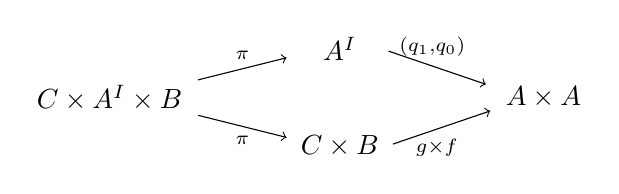
\begin{tikzpicture}[x=1.6em,y=1.6em]
  \node (CAB) at (0,0) {$C\times A^{\hciso}\times B$};
  \node (AI)  at (5.2,1.1) {$A^{\hciso}$};
  \node (CB)  at (5.2,-1.1) {$C\times B$};
  \node (AA)  at (9.8,0) {$A\times A$};
  \draw[->] (2.0,0.4) -- node[above,pos=0.5]{$\scriptstyle\pi$} (4.0,0.9);
  \draw[->] (2.0,-0.4) -- node[below,pos=0.5]{$\scriptstyle\pi$} (4.0,-0.9);
  \draw[->] (6.3,1.05) -- node[above,pos=0.45]{$\scriptstyle(q_{1},q_{0})$} (8.5,0.3);
  \draw[->] (6.4,-1.05) -- node[below,pos=0.45]{$\scriptstyle g\times f$} (8.6,-0.3);
\end{tikzpicture}
\end{center}
其中映射 $(q_{1},q_{0})\colon A^{\hciso}\to A\times A$ 由沿端点包含
$\qcOne+\qcOne=\partial\hciso\hookrightarrow\hciso$ 作限制而定义。在一个%
\trInfinityCosmos{}中，这一映射是一条\trIsofibration，而定义同构逗号对象的
等化子由\trPullback{} \eqref{eq:iso-comma-pullback} 计算。

\begin{rveq}\label{eq:iso-comma-pullback}
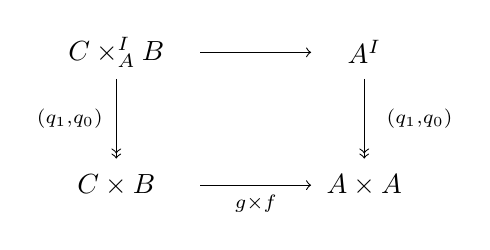
\begin{tikzpicture}[x=1.6em,y=1.6em]
  \node (CIB) at (0,1.5) {$C\times^{\hciso}_{A}B$};
  \node (AI)  at (5.6,1.5) {$A^{\hciso}$};
  \node (CB)  at (0,-1.5) {$C\times B$};
  \node (AA)  at (5.6,-1.5) {$A\times A$};
  \draw[->] (1.9,1.5) -- (4.4,1.5);
  \draw[->>] (0,0.9) -- (0,-0.9);
  \node at (0.5,0.7) {$\scriptstyle\lrcorner$};
  \node at (-1.05,0) {$\scriptstyle(q_{1},q_{0})$};
  \draw[->>] (5.6,0.9) -- (5.6,-0.9);
  \node at (6.85,0) {$\scriptstyle(q_{1},q_{0})$};
  \draw[->] (1.9,-1.5) -- node[below]{$\scriptstyle g\times f$} (4.4,-1.5);
\end{tikzpicture}
\end{rveq}

\begin{lemma}\label{lem:iso-commas-flexible}
同构逗号对象是\trFlexibleWeightedLimit{}，从而特别地存在于任何\trInfinityCosmos{}中。
\end{lemma}

\begin{proof}
把\trCospan{}\trCategory{} $\csp$ 中的对象写作 $b\to a\leftarrow c$，权 $W_{\times}$ 由如下%
\trPushout{}构造：
\begin{center}
\begin{tikzpicture}[x=1.6em,y=1.7em]
  \node (dIa) at (0,1.5) {$\partial\hciso\times\csp(a,-)$};
  \node (bc)  at (7.6,1.5) {$\csp(b,-)\sqcup\csp(c,-)$};
  \node (Ia)  at (0,-1.5) {$\hciso\times\csp(a,-)$};
  \node (W)   at (7.6,-1.5) {$W_{\times}$};
  \draw[->] (2.85,1.5) -- (5.2,1.5);
  \draw[right hook->] (0,0.85) -- (0,-0.85);
  \draw[right hook->] (7.6,0.85) -- (7.6,-0.85);
  \draw[->] (2.85,-1.5) -- (6.2,-1.5);
  \node at (6.9,-0.85) {$\scriptstyle\ulcorner$};
\end{tikzpicture}
\end{center}
其中粘贴映射选出\trCospan{}中的两支箭头。作为一个射影胞腔复形，$W_{\times}$ 由
$b$ 处的一个射影 0-胞腔、$c$ 处的一个射影 0-胞腔、以及对每个 $k>0$ 在 $a$ 处
的两个射影 $k$-胞腔构造而成，后者对应于 $\hciso$ 的诸非退化单纯形。如%
\cref{rem:projective-cell-complexes}所述，这些可以一次性全部附接。如此便见
$W_{\times}$ 是一个柔性权，于是\cref{prop:flexible-weights-homotopical}(i)
告诉我们同构逗号对象存在于任何\trInfinityCosmos{}中——这一事实从\trPullback
\eqref{eq:iso-comma-pullback} 中也显而易见。
\end{proof}

\begin{remark}\label{rem:iso-comma-cone}
在一个\trInfinityCosmos{}的\trHomotopyTwoCategory{}中，有一支典范的可逆
2-胞腔定义出\textbf{同构逗号锥}（iso-comma cone）：
\begin{center}
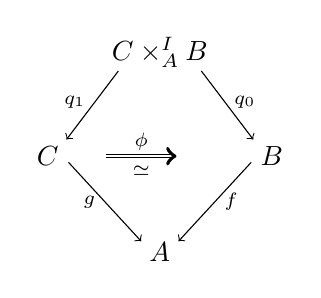
\begin{tikzpicture}[x=1.5em,y=1.5em]
  \node (CIB) at (2.7,1.8) {$C\times^{\hciso}_{A}B$};
  \node (C) at (0,-0.7) {$C$};
  \node (B) at (5.4,-0.7) {$B$};
  \node (A) at (2.7,-3.0) {$A$};
  \draw[->] (1.7,1.35) -- node[left,pos=0.45]{$\scriptstyle q_{1}$} (0.45,-0.3);
  \draw[->] (3.7,1.35) -- node[right,pos=0.45]{$\scriptstyle q_{0}$} (4.95,-0.3);
  \draw[->] (0.5,-0.85) -- node[left,pos=0.5]{$\scriptstyle g$} (2.25,-2.75);
  \draw[->] (4.9,-0.85) -- node[right,pos=0.5]{$\scriptstyle f$} (3.15,-2.75);
  \draw[double,->] (1.4,-0.7) -- (3.1,-0.7);
  \node at (2.25,-0.35) {$\scriptstyle\phi$};
  \node at (2.25,-1.05) {$\scriptstyle\simeq$};
\end{tikzpicture}
\end{center}
它享有一条与命题 3.4.6 所给出的逗号锥相类似的弱\trUniversalProperty{}（见
[110, §3]）。其证明用到了 $A^{\hciso}$ 是\trHomotopyTwoCategory{}中的弱
$\hciso$-\trCotensor{}这一事实 [108, 3.3.13]。

我们为同构逗号所选的记号有意与\trPullback{}的通常记号相类似。在一个\trInfinityCosmos{}%
中，同构逗号可用于计算这样一些\trDiagram{}的「同伦拉回」：其中没有一条映射是%
\trIsofibration。当\trCospan{}中至少有一条映射是\trIsofibration{}时，同构逗号等价
于锥形拉回。
\end{remark}

\begin{lemma}[同构逗号与拉回]\label{lem:iso-commas-pullbacks}
对于\trInfinityCosmos{}中涉及至少一条\trIsofibration{}的任何\trCospan，\trPullback{}与
同构逗号等价。更精确地说，给定如下左图所示的\trPullback{}方块与如下右图所示的同构逗号
方块
\begin{center}
\begin{tikzpicture}[x=1.5em,y=1.5em]
  \begin{scope}[shift={(0,0)}]
  \node (P) at (0,1.5) {$P$};
  \node (B) at (3.8,1.5) {$B$};
  \node (C) at (0,-1.5) {$C$};
  \node (A) at (3.8,-1.5) {$A$};
  \draw[->] (0.55,1.5) -- node[above]{$\scriptstyle b$} (3.2,1.5);
  \draw[->>] (0,0.9) -- (0,-0.9);
  \node at (0.5,0.7) {$\scriptstyle\lrcorner$};
  \node at (-0.45,0) {$\scriptstyle c$};
  \draw[->>] (3.8,0.9) -- (3.8,-0.9);
  \node at (4.25,0) {$\scriptstyle f$};
  \draw[->] (0.55,-1.5) -- node[below]{$\scriptstyle g$} (3.2,-1.5);
  \node at (5.9,0) {，};
  \end{scope}
  \begin{scope}[shift={(7.8,0)}]
  \node (CIB) at (1.3,1.5) {$C\times^{\hciso}_{A}B$};
  \node (B) at (5.1,1.5) {$B$};
  \node (C) at (0,-1.5) {$C$};
  \node (A) at (5.1,-1.5) {$A$};
  \draw[->>] (3.0,1.5) -- node[above]{$\scriptstyle q_{0}$} (4.55,1.5);
  \draw[->>] (0.85,1.1) -- node[left,pos=0.5]{$\scriptstyle q_{1}$} (0.25,-0.9);
  \draw[->>] (5.1,0.9) -- (5.1,-0.9);
  \node at (5.55,0) {$\scriptstyle f$};
  \draw[->] (0.55,-1.5) -- node[below]{$\scriptstyle g$} (4.5,-1.5);
  \node at (2.2,0.05) {$\scriptstyle\phi$};
  \draw[double,->] (1.75,-0.35) -- (2.65,-0.35);
  \node at (2.2,-0.75) {$\scriptstyle\simeq$};
  \end{scope}
\end{tikzpicture}
\end{center}
则 $P\simeq C\times^{\hciso}_{A}B$ 在 $C$ 之上成立，且在 $B$ 之上至相差同构。
\end{lemma}

\begin{proof}
把引理 1.2.19 应用于函子 $b\colon P\to B$，我们可以把跨度
$(c,b)\colon P\to C\times B$ 替换为一个两腿皆为\trIsofibration{}的跨度
$(cq,p)\colon Pb\to C\times B$，后者经一个等价 $s\colon P\Rightarrow Pb$ 与原
跨度相关联，该等价在 $C$ 之上严格成立、在 $B$ 之上至相差同构。我们断言：在
$f$ 是\trIsofibration{}的假设下，这条新跨度等价于同构逗号跨度。
为看清这一点，注意 (1.2.20) 中构造的因子分解实际上是用一个同构逗号定义的，该
同构逗号经下左图顶部的方块中的\trPullback{}构造。由于映射 $b$ 本身由一个\trPullback{}定义，下
左图的底部方块也是一个\trPullback，从而定义出左侧的\trPullback{}矩形：
\begin{center}
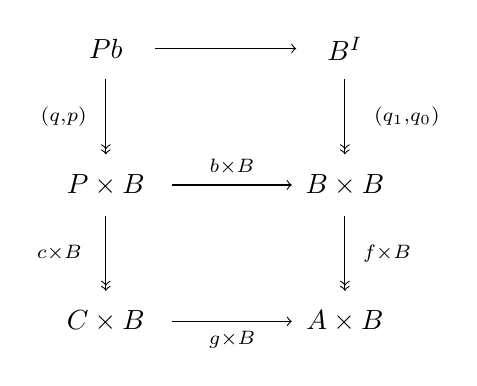
\begin{tikzpicture}[x=1.6em,y=1.7em]
  \node (Pb) at (0,2.9) {$Pb$};
  \node (BI) at (5.4,2.9) {$B^{\hciso}$};
  \node (PB) at (0,0) {$P\times B$};
  \node (BB) at (5.4,0) {$B\times B$};
  \node (CB) at (0,-2.9) {$C\times B$};
  \node (AB) at (5.4,-2.9) {$A\times B$};
  \draw[->] (1.1,2.9) -- (4.3,2.9);
  \draw[->>] (0,2.25) -- (0,0.65);
  \node at (0.5,2.05) {$\scriptstyle\lrcorner$};
  \node at (-0.95,1.45) {$\scriptstyle(q,p)$};
  \draw[->>] (5.4,2.25) -- (5.4,0.65);
  \node at (6.8,1.45) {$\scriptstyle(q_{1},q_{0})$};
  \draw[->] (1.5,0) -- node[above]{$\scriptstyle b\times B$} (4.2,0);
  \draw[->>] (0,-0.65) -- (0,-2.25);
  \node at (0.5,-2.05) {$\scriptstyle\lrcorner$};
  \node at (-1.05,-1.45) {$\scriptstyle c\times B$};
  \draw[->>] (5.4,-0.65) -- (5.4,-2.25);
  \node at (6.35,-1.45) {$\scriptstyle f\times B$};
  \draw[->] (1.5,-2.9) -- node[below]{$\scriptstyle g\times B$} (4.2,-2.9);
\end{tikzpicture}
\end{center}
现在，同构逗号由一个类似的\trPullback{}矩形构造，如下右图所示。由于 $f$ 是%
\trIsofibration，引理 1.2.14 告诉我们：$i_{0}\colon\qcOne\hookrightarrow\hciso$ 与
$f\colon B\twoheadrightarrow A$ 的 Leibniz 张量
$i_{0}\hat{\times}f\colon B^{\hciso}\twoheadrightarrow A\times^{\hciso}_{A}B$
是一个\trTrivialFibration。这一等价与到 $A\times B$ 的诸投影交换，于是映射
$(cq,p)\colon Pb\twoheadrightarrow C\times B$ 与
$(q_{1},q_{0})\colon C\times^{\hciso}_{A}B\twoheadrightarrow C\times B$——作
为沿 $g\times B$ 拉回一对彼此等价的\trIsofibration{}而定义——如所断言是等价
的。
\begin{center}
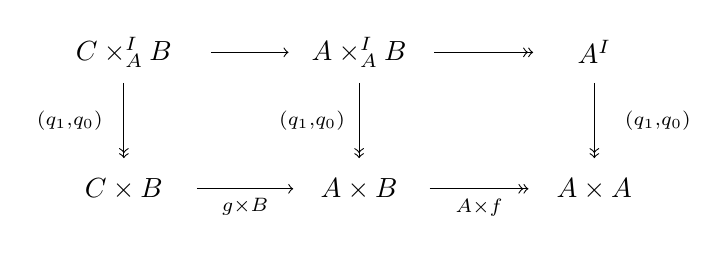
\begin{tikzpicture}[x=1.7em,y=1.7em]
  \node (CIB) at (0,2.9) {$C\times^{\hciso}_{A}B$};
  \node (AIB) at (5.0,2.9) {$A\times^{\hciso}_{A}B$};
  \node (AI)  at (10.0,2.9) {$A^{\hciso}$};
  \node (CB)  at (0,0) {$C\times B$};
  \node (AB)  at (5.0,0) {$A\times B$};
  \node (AA)  at (10.0,0) {$A\times A$};
  \draw[->] (1.85,2.9) -- (3.5,2.9);
  \draw[->>] (6.6,2.9) -- (8.7,2.9);
  \draw[->>] (0,2.25) -- (0,0.65);
  \node at (0.5,2.05) {$\scriptstyle\lrcorner$};
  \node at (-1.15,1.45) {$\scriptstyle(q_{1},q_{0})$};
  \draw[->>] (5.0,2.25) -- (5.0,0.65);
  \node at (5.5,2.05) {$\scriptstyle\lrcorner$};
  \node at (4.0,1.45) {$\scriptstyle(q_{1},q_{0})$};
  \draw[->>] (10.0,2.25) -- (10.0,0.65);
  \node at (11.35,1.45) {$\scriptstyle(q_{1},q_{0})$};
  \draw[->] (1.55,0) -- node[below]{$\scriptstyle g\times B$} (3.6,0);
  \draw[->>] (6.5,0) -- node[below]{$\scriptstyle A\times f$} (8.6,0);
\end{tikzpicture}
\end{center}
\end{proof}

现在我们为如下\trDiagram{}引入一个柔性权：由 0-箭头的可数塔给出的\trDiagram，
其锥形状在每支生成箭头之上的三角形中都有一个\trHomotopyCoherentIsomorphism。

\begin{definition}[同构塔]\label{def:iso-towers}
回忆范畴 $\omega$：其对象为自然数，其态射由每个 $n$ 处的映射
$\imath_{n,n+1}\colon n\to n+1$ 自由生成。$\omega^{\mathrm{op}}$ 形状的%
\trDiagram
\[
F:=\quad
\cdots\xrightarrow{\ f_{n+2,n+1}\ }F_{n+1}
\xrightarrow{\ f_{n+1,n}\ }F_{n}
\xrightarrow{\ f_{n,n-1}\ }\cdots
\xrightarrow{\ f_{2,1}\ }F_{1}
\xrightarrow{\ f_{1,0}\ }F_{0}
\]
在单纯富集且余张量化的\trCategory{}中的\textbf{同构塔}（iso-tower），是以%
\trDiagram{} $W^{\leftarrow}\colon\omega^{\mathrm{op}}\to sSet$ 加权的%
\trLimit，该权由 $sSet^{\omega^{\mathrm{op}}}$ 中的\trPushout{}定义：
\begin{rveq}\label{eq:iso-tower-weight}
\begin{tikzpicture}[x=1.6em,y=1.8em]
  \node (dI) at (0,1.5) {$\coprod_{n\in\omega}\partial\hciso\times\omega(-,n)$};
  \node (copr) at (9.6,1.5) {$\coprod_{m\in\omega}\omega(-,m)$};
  \node (I) at (0,-1.5) {$\coprod_{n\in\omega}\hciso\times\omega(-,n)$};
  \node (W) at (9.6,-1.5) {$W^{\leftarrow}$};
  \draw[->] (4.9,1.5) -- node[above]{$\scriptstyle(\mathrm{id}_{n},\imath_{n,n+1})$} (7.3,1.5);
  \draw[right hook->] (0,0.9) -- (0,-0.9);
  \draw[right hook->] (9.6,0.9) -- (9.6,-0.9);
  \draw[->] (4.9,-1.5) -- (7.9,-1.5);
  \node at (8.9,-0.8) {$\scriptstyle\ulcorner$};
\end{tikzpicture}
\end{rveq}
\end{definition}

由定义 A.6.1(ii)，在\trInfinityCosmos{}中，$F$ 的同构塔由\trPullback{}构造：
\begin{rveq}\label{eq:iso-tower-pullback}
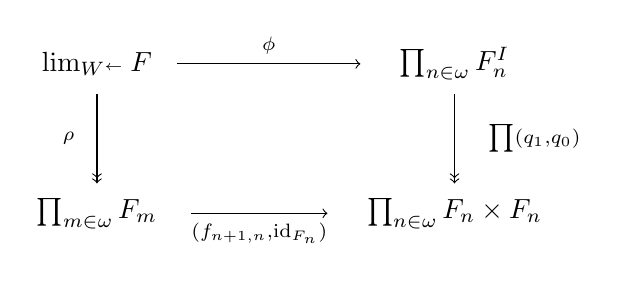
\begin{tikzpicture}[x=1.7em,y=1.8em]
  \node (limF) at (0,1.5) {$\lim_{W^{\leftarrow}}F$};
  \node (prodI) at (7.6,1.5) {$\prod_{n\in\omega}F^{\hciso}_{n}$};
  \node (prodF) at (0,-1.5) {$\prod_{m\in\omega}F_{m}$};
  \node (prodFF) at (7.6,-1.5) {$\prod_{n\in\omega}F_{n}\times F_{n}$};
  \draw[->] (1.7,1.5) -- node[above]{$\scriptstyle\phi$} (5.6,1.5);
  \draw[->>] (0,0.9) -- (0,-0.9);
  \node at (0.5,0.65) {$\scriptstyle\lrcorner$};
  \node at (-0.6,0) {$\scriptstyle\rho$};
  \draw[->>] (7.6,0.9) -- (7.6,-0.9);
  \node at (9.3,0) {$\scriptstyle\prod(q_{1},q_{0})$};
  \draw[->] (2.0,-1.5) -- node[below]{$\scriptstyle(f_{n+1,n},\mathrm{id}_{F_{n}})$} (4.9,-1.5);
\end{tikzpicture}
\end{rveq}

极限锥由一支 0-箭头 $\rho_{n}\colon\lim_{W^{\leftarrow}}F\to F_{n}$（对每个
$n\in\omega$）连同 $\omega^{\mathrm{op}}$-指标\trDiagram{}中每支生成箭头
$F_{n+1}\to F_{n}$ 之上三角形里的一个\trHomotopyCoherentIsomorphism{}
$\phi_{n}$ 一起生成。

\begin{lemma}\label{lem:iso-towers-flexible}
同构塔是\trFlexibleWeightedLimit{}，从而特别地存在于任何\trInfinityCosmos{}中。
\end{lemma}

\begin{proof}
权 $W^{\leftarrow}$ 是一个射影胞腔复形，其构造方式是：在每个 $n\in\omega$ 处
附接一个射影 0-胞腔——形成 \eqref{eq:iso-tower-weight} 右上角的\trCoproduct——然后对
$\hciso$ 的每个非退化的 $k$-单纯形（$k>0$），在每个 $n\in\omega$ 处附接一个
射影 $k$-胞腔。对固定 $n\in\omega$ 的诸射影 $k$-胞腔，与其逐一依序附接，不如
按\cref{rem:projective-cell-complexes}，通过取由映射
$\partial\hciso\times\omega(-,n)\hookrightarrow\hciso\times\omega(-,n)$ 定义的
「$n$ 处的广义射影胞腔」的单一\trPushout，将它们一次性全部附接。这些正是以
\eqref{eq:iso-tower-weight} 左侧竖直边出现的那些映射。现在，
\cref{prop:flexible-weights-homotopical}(i) 或公式 \eqref{eq:iso-tower-pullback}
都清楚地表明：这类对象存在于任何\trInfinityCosmos{}中。
\end{proof}

正如同构逗号之于\trPullback，同构塔给出了一种计算由任意映射构成的\trDiagram{}之逆向
极限的方法。当这些映射是\trIsofibration{}时，同构塔等价于锥形极限。

\begin{lemma}[同构塔与逆向极限]\label{lem:iso-towers-inverse-limits}
\trInfinityCosmos{}中\trIsofibration{}之可数塔的逆向极限，等价于该塔的同构拉回。
\footnote{译注：原书此处作「iso-pullback」（同构拉回），全书并未定义这一术语；
据证明内容，所指应为以 $W^{\leftarrow}$ 加权的极限（同构塔）。此处照录原书
面貌。}
\end{lemma}

\begin{proof}
我们将重新安排极限 \eqref{eq:iso-tower-pullback}，在\trInfinityCosmos{}
$\mathcal{K}$ 中把同构塔 $\lim_{W^{\leftarrow}}F$ 构造为\trIsofibration{}的一
座可数塔 $P\colon\omega^{\mathrm{op}}\to\mathcal{K}$ 的逆向极限，后者逐点等价
于\trIsofibration{}之塔 $F\colon\omega^{\mathrm{op}}\to\mathcal{K}$\footnote{原
书下方显示式中 $P_{n+1}$ 列与 $P_{n}$ 列之竖直标签均印作 $e_{n}$，前者按上下
文（$e_{n}\colon P_{n}\twoheadrightarrow F_{n}$）疑为 $e_{n+1}$ 之误，径改。——译者注}：
\begin{rveq}\label{eq:iso-tower-rearrangement}
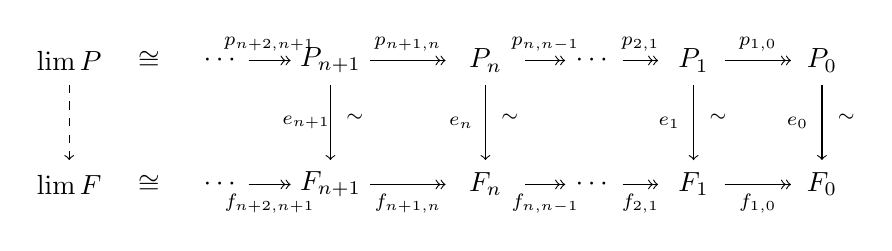
\begin{tikzpicture}[x=1.6em,y=1.6em]
  \node (lP)  at (0,1.4) {$\lim P$};
  \node (cP)  at (1.8,1.4) {$\cong$};
  \node (d1)  at (3.4,1.4) {$\cdots$};
  \node (Pn1) at (5.9,1.4) {$P_{n+1}$};
  \node (Pn)  at (9.4,1.4) {$P_{n}$};
  \node (d2)  at (11.8,1.4) {$\cdots$};
  \node (P1)  at (14.1,1.4) {$P_{1}$};
  \node (P0)  at (17.0,1.4) {$P_{0}$};
  \draw[->>] (4.05,1.4) -- node[above]{$\scriptstyle p_{n+2,n+1}$} (5.0,1.4);
  \draw[->>] (6.8,1.4) -- node[above]{$\scriptstyle p_{n+1,n}$} (8.5,1.4);
  \draw[->>] (10.3,1.4) -- node[above]{$\scriptstyle p_{n,n-1}$} (11.2,1.4);
  \draw[->>] (12.5,1.4) -- node[above]{$\scriptstyle p_{2,1}$} (13.3,1.4);
  \draw[->>] (14.8,1.4) -- node[above]{$\scriptstyle p_{1,0}$} (16.3,1.4);
  \node (lF)  at (0,-1.4) {$\lim F$};
  \node (cF)  at (1.8,-1.4) {$\cong$};
  \node (d3)  at (3.4,-1.4) {$\cdots$};
  \node (Fn1) at (5.9,-1.4) {$F_{n+1}$};
  \node (Fn)  at (9.4,-1.4) {$F_{n}$};
  \node (d4)  at (11.8,-1.4) {$\cdots$};
  \node (F1)  at (14.1,-1.4) {$F_{1}$};
  \node (F0)  at (17.0,-1.4) {$F_{0}$};
  \draw[->>] (4.05,-1.4) -- node[below]{$\scriptstyle f_{n+2,n+1}$} (5.0,-1.4);
  \draw[->>] (6.8,-1.4) -- node[below]{$\scriptstyle f_{n+1,n}$} (8.5,-1.4);
  \draw[->>] (10.3,-1.4) -- node[below]{$\scriptstyle f_{n,n-1}$} (11.2,-1.4);
  \draw[->>] (12.5,-1.4) -- node[below]{$\scriptstyle f_{2,1}$} (13.3,-1.4);
  \draw[->>] (14.8,-1.4) -- node[below]{$\scriptstyle f_{1,0}$} (16.3,-1.4);
  \draw[->] (5.9,0.85) -- (5.9,-0.85);
  \node at (6.45,0.1) {$\scriptstyle\sim$};
  \node at (5.35,0) {$\scriptstyle e_{n+1}$};
  \draw[->] (9.4,0.85) -- (9.4,-0.85);
  \node at (9.95,0.1) {$\scriptstyle\sim$};
  \node at (8.85,0) {$\scriptstyle e_{n}$};
  \draw[->] (14.1,0.85) -- (14.1,-0.85);
  \node at (14.65,0.1) {$\scriptstyle\sim$};
  \node at (13.55,0) {$\scriptstyle e_{1}$};
  \draw[->] (17.0,0.85) -- (17.0,-0.85);
  \node at (17.55,0.1) {$\scriptstyle\sim$};
  \node at (16.45,0) {$\scriptstyle e_{0}$};
  \draw[->,dashed] (0,0.85) -- (0,-0.85);
\end{tikzpicture}
\end{rveq}
由\trIsofibration{}之\trDiagram{}的逆向极限的等价不变性可知，极限
$\lim_{W^{\leftarrow}}F\cong\lim P$ 与 $\lim F$ 等价，正如所断言。

∞-范畴 $P_{n}$ 定义为\trDiagram{} \eqref{eq:iso-tower-pullback} 的截断版本的
锥形极限。首先定义 $P_{0}:=F_{0}$ 且 $e_{0}$ 为恒同，然后经\trPullback{}定义 $P_{1}$、
$p_{1,0}$ 与 $e_{1}$：
\begin{center}
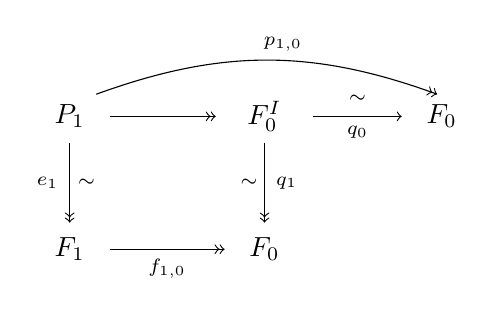
\begin{tikzpicture}[x=1.6em,y=1.6em]
  \node (P1) at (0,1.5) {$P_{1}$};
  \node (FI) at (4.4,1.5) {$F^{\hciso}_{0}$};
  \node (F0) at (8.4,1.5) {$F_{0}$};
  \node (F1) at (0,-1.5) {$F_{1}$};
  \node (F0b) at (4.4,-1.5) {$F_{0}$};
  \draw[->>] (0.9,1.5) -- (3.3,1.5);
  \draw[->] (5.5,1.5) -- node[below]{$\scriptstyle q_{0}$} (7.5,1.5);
  \node at (6.5,1.9) {$\scriptstyle\sim$};
  \draw[->>] (0.6,2.0) to[bend left=20] node[above,pos=0.55]{$\scriptstyle p_{1,0}$} (8.3,2.0);
  \draw[->>] (0,0.9) -- (0,-0.9);
  \node at (0.5,0.7) {$\scriptstyle\lrcorner$};
  \node at (-0.5,0) {$\scriptstyle e_{1}$};
  \node at (0.38,0) {$\scriptstyle\sim$};
  \draw[->>] (4.4,0.9) -- (4.4,-0.9);
  \node at (4.9,0) {$\scriptstyle q_{1}$};
  \node at (4.05,0) {$\scriptstyle\sim$};
  \draw[->>] (0.9,-1.5) -- node[below]{$\scriptstyle f_{1,0}$} (3.5,-1.5);
\end{tikzpicture}
\end{center}
注意 $P_{1}\cong F_{1}\times^{\hciso}_{F_{0}}F_{0}$ 计算了由
$\mathrm{id}_{F_{0}}$ 与 $f_{1,0}$ 给出的\trCospan{}的同构逗号对象。

现在用复合\trPullback{}定义 $P_{2}$、$p_{2,1}$ 与 $e_{2}$：
\begin{center}
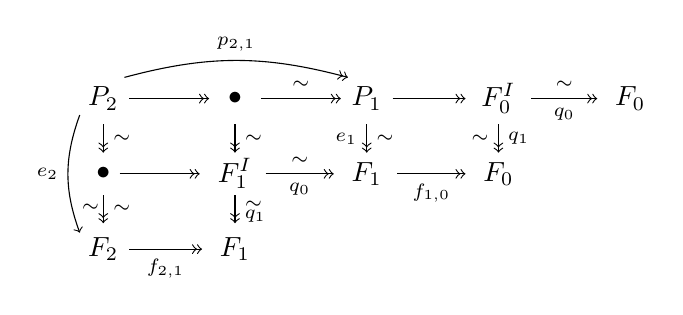
\begin{tikzpicture}[x=1.7em,y=1.7em]
  \node (P2)  at (0,1.6)    {$P_{2}$};
  \node (Dt)  at (2.8,1.6)  {$\bullet$};
  \node (P1)  at (5.6,1.6)  {$P_{1}$};
  \node (FI0) at (8.4,1.6)  {$F^{\hciso}_{0}$};
  \node (F0t) at (11.2,1.6) {$F_{0}$};
  \node (Dm)  at (0,0)      {$\bullet$};
  \node (FI1) at (2.8,0)    {$F^{\hciso}_{1}$};
  \node (F1m) at (5.6,0)    {$F_{1}$};
  \node (F0m) at (8.4,0)    {$F_{0}$};
  \node (F2)  at (0,-1.6)   {$F_{2}$};
  \node (F1b) at (2.8,-1.6) {$F_{1}$};
  \draw[->>] (0.55,1.6) -- (2.25,1.6);
  \draw[->>] (3.35,1.6) -- node[above]{$\scriptstyle\sim$} (5.05,1.6);
  \draw[->>] (6.15,1.6) -- (7.7,1.6);
  \draw[->>] (9.1,1.6) -- node[above]{$\scriptstyle\sim$} node[below]{$\scriptstyle q_{0}$} (10.5,1.6);
  \draw[->>] (0.35,0) -- (2.05,0);
  \draw[->>] (3.45,0) -- node[above]{$\scriptstyle\sim$} node[below]{$\scriptstyle q_{0}$} (4.9,0);
  \draw[->>] (6.25,0) -- node[below]{$\scriptstyle f_{1,0}$} (7.7,0);
  \draw[->>] (0.55,-1.6) -- node[below]{$\scriptstyle f_{2,1}$} (2.1,-1.6);
  \draw[->>] (0,1.05) -- node[right]{$\scriptstyle\sim$} (0,0.45);
  \draw[->>] (2.8,1.05) -- node[right]{$\scriptstyle\sim$} (2.8,0.45);
  \draw[->>] (5.6,1.05) -- node[left]{$\scriptstyle e_{1}$} node[right]{$\scriptstyle\sim$} (5.6,0.45);
  \draw[->>] (8.4,1.05) -- node[left]{$\scriptstyle\sim$} node[right]{$\scriptstyle q_{1}$} (8.4,0.45);
  \draw[->>] (0,-0.45) -- node[right]{$\scriptstyle\sim$} (0,-1.05);
  \draw[->>] (2.8,-0.45) -- node[right,pos=0.35]{$\scriptstyle\sim$} node[right,pos=0.75]{$\scriptstyle q_{1}$} (2.8,-1.05);
  \draw[->>] (0.45,2.05) to[bend left=15] node[above,pos=0.5]{$\scriptstyle p_{2,1}$} (5.2,2.05);
  \draw[->] (-0.5,1.25) to[bend right=20] node[left,pos=0.5]{$\scriptstyle e_{2}$} node[right,pos=0.8]{$\scriptstyle\sim$} (-0.5,-1.25);
  \node at (0.6,1.15) {$\scriptstyle\lrcorner$};
  \node at (3.4,1.15) {$\scriptstyle\lrcorner$};
  \node at (6.2,1.15) {$\scriptstyle\lrcorner$};
  \node at (0.6,-0.45) {$\scriptstyle\lrcorner$};
\end{tikzpicture}
\end{center}

依归纳继续，$P_{n}$、$p_{n,n-1}$ 与 $e_{n}$ 的定义方式是：把图表
\begin{center}
\begin{tikzpicture}[x=1.6em,y=1.6em]
  \node (FIm1) at (2.0,1.5) {$F^{\hciso}_{n-1}$};
  \node (Fm1) at (6.6,1.5) {$F_{n-1}$};
  \node (Fn) at (-1.2,-1.5) {$F_{n}$};
  \node (Fm1b) at (2.0,-1.5) {$F_{n-1}$};
  \draw[->>] (3.2,1.5) -- node[below]{$\scriptstyle q_{0}$} (5.4,1.5);
  \node at (4.3,1.95) {$\scriptstyle\sim$};
  \draw[->>] (2.0,0.9) -- (2.0,-0.9);
  \node at (1.6,0) {$\scriptstyle\sim$};
  \node at (2.5,0) {$\scriptstyle q_{1}$};
  \draw[->>] (-0.45,-1.5) -- node[below]{$\scriptstyle f_{n,n-1}$} (1.15,-1.5);
\end{tikzpicture}
\end{center}
附加到定义 $P_{n-1}$ 的极限锥上，并取这张复合图表的极限。在极限中，这张复合
图表是 \eqref{eq:iso-tower-pullback} 的一个展开。于是
$\lim_{W^{\leftarrow}}F\cong\lim P$。

剩下要用映射 $e_{n}\colon P_{n}\twoheadrightarrow F_{n}$ 来比较 $\lim P$ 与
$\lim F$。刚才给出的构造有一个小问题：它定义出的图表
\eqref{eq:iso-tower-rearrangement} 中，每个方块只在同构的意义下交换——由映射
$P_{n}\to F^{\hciso}_{n-1}$ 编码的那个同构——而非严格交换。但由于诸映射
$f_{n+1,n}$ 是\trIsofibration，这不成问题。栖居于方块
$e_{0}p_{1,0}\cong f_{1,0}e_{1}$ 中的那个同构可以沿 $f_{1,0}$ 提升，从而定义
出一支与 $e_{1}$ 同构的新映射 $e'_{1}\colon P_{1}\twoheadrightarrow F_{1}$。
由练习 1.4.ii，这支 $e'_{1}$ 于是仍是一个\trEquivalence（尽管不再必然是%
\trTrivialFibration），所以我们把 $e_{1}$ 替换为 $e'_{1}$，然后依归纳继续，把
方块 $e'_{1}p_{2,1}\cong f_{2,1}e_{2}$ 中的同构逐一提升消去。

由于\trIsofibration{}之塔的逆向极限在\trEquivalence{}下不变（命题 C.1.15），
可知 $\lim P\cong\lim F$。由构造 $\lim P\cong\lim_{W^{\leftarrow}}F$，于是
$\lim_{W^{\leftarrow}}F\simeq\lim F$，这正是所要证明的。
\end{proof}

\subsection*{练习}

\begin{exercise}\label{ex:wide-pullbacks}
（[112, 2.2.2]）试证明：\trInfinityCosmos{}容有\textbf{宽拉回}（wide
pullbacks）：如下形状的有限或可数\trDiagram{}的极限
\begin{center}
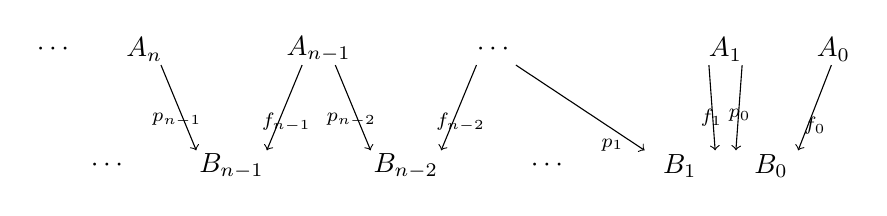
\begin{tikzpicture}[x=1.5em,y=1.4em]
  \node (ldots) at (-2.2,1.4) {$\cdots$};
  \node (An) at (0,1.4) {$A_{n}$};
  \node (Anm1) at (4.2,1.4) {$A_{n-1}$};
  \node (Adots) at (8.4,1.4) {$\cdots$};
  \node (A1) at (14.0,1.4) {$A_{1}$};
  \node (A0) at (16.6,1.4) {$A_{0}$};
  \node (bdots1) at (-0.9,-1.6) {$\cdots$};
  \node (Bnm1) at (2.1,-1.6) {$B_{n-1}$};
  \node (Bnm2) at (6.3,-1.6) {$B_{n-2}$};
  \node (bdots2) at (9.7,-1.6) {$\cdots$};
  \node (B1) at (12.9,-1.6) {$B_{1}$};
  \node (B0) at (15.1,-1.6) {$B_{0}$};
  \draw[->] (0.4,1.0) -- node[below,pos=0.45]{$\scriptstyle p_{n-1}$} (1.25,-1.2);
  \draw[->] (3.8,1.0) -- node[below,pos=0.45]{$\scriptstyle f_{n-1}$} (2.95,-1.2);
  \draw[->] (4.6,1.0) -- node[below,pos=0.45]{$\scriptstyle p_{n-2}$} (5.45,-1.2);
  \draw[->] (8.0,1.0) -- node[below,pos=0.45]{$\scriptstyle f_{n-2}$} (7.15,-1.2);
  \draw[->] (8.95,1.0) -- node[below,pos=0.75]{$\scriptstyle p_{1}$} (12.05,-1.2);
  \draw[->] (13.6,1.0) -- node[below,pos=0.4]{$\scriptstyle f_{1}$} (13.75,-1.2);
  \draw[->] (14.4,1.0) -- node[below,pos=0.4]{$\scriptstyle p_{0}$} (14.25,-1.2);
  \draw[->] (16.55,1.0) -- node[below,pos=0.5]{$\scriptstyle f_{0}$} (15.75,-1.2);
\end{tikzpicture}
\end{center}
并且它们的构造在\trDiagram{}之间的逐点\trEquivalence{}下不变。
\end{exercise}

